\section{Theoretical Analysis}
\label{sec:analysis}

\subsection{Nodal Method for t $<$ 0}

The objective of this method is to  determine every node voltage. To do this we have to first number nodes arbitrarily, assign potential 0V (Ground) to one of the nodes (node 4 in this case), and then calculate all the voltages. We had 8 unknown variables, so we determined 8 independent equations. Before t $<$ 0s, $v(s) = V_s$ (constant), hence the capacitor behaves as an open-circuit ($I_x$ = 0). The equations were rearranged in the matrix form below, in order to find the solution using Octave math tools. The circuit that we analysed in this section, was the circuit 1 of the introduction.The results are shown in the tables below.

\begin{center}
$\begin{bmatrix}
1 & 0 & 0 & 0 & 0 & 0 & 0 & 0\\
-G_1 & G_1+G_2+G_3 & -G_2 & 0 & -G_3 & 0 & 0 & 0\\
0 & -K_b-G_2 & G_2 & 0 & K_b & 0 & 0 & 0\\
0 & 0 & 0 & 1 & 0 & 0 & 0 & 0\\
0 & -G_3 & 0 & -G_4 & G_3+G_4+G_5 & -G_5 & -G_7 & G_7\\
0 & K_b & 0 & 0 & -K_b-G_5 & G_5 & 0 & 0 \\
0 & 0 & 0 & -G_6 & 0 & 0 & G_6+G_7 & -G_7\\
0 & 0 & 0 & K_d*G_6 & -1 & 0 & -K_d*G_6 & 1
\end{bmatrix}$
$\begin{bmatrix}
V_1 \\ V_2 \\ V_3 \\ V_4 \\ V_5 \\ V_6 \\ V_7 \\ V_8
\end{bmatrix}$
= 
$\begin{bmatrix}
V_s \\ 0 \\ 0 \\ 0 \\ 0 \\ 0 \\ 0 \\ 0
\end{bmatrix}$
\end{center}

\begin{table}[h]
\centering
\begin{tabularx}{0.6\textwidth} {
  | >{\raggedright\arraybackslash}X
  | >{\raggedleft\arraybackslash}X | }
 \hline
V1 & 5.114229e+00 V\\ \hline
V2 & 4.873694e+00 V\\ \hline
V3 & 4.380386e+00 V\\ \hline
V4 & 0.000000e+00 V\\ \hline
V5 & 4.906396e+00 V\\ \hline
V6 & 5.644102e+00 V\\ \hline
V7 & -1.935730e+00 V\\ \hline
V8 & -2.918905e+00 V\\ \hline

\end{tabularx}
\caption{Theoretical Nodal Voltages expressed in V}
\end{table}

\begin{table}[h]
\centering
\begin{tabularx}{0.6\textwidth} {
  | >{\raggedright\arraybackslash}X
  | >{\raggedleft\arraybackslash}X | }
 \hline
I1 & -2.293000e-04 A\\ \hline
I2 & -2.399863e-04 A\\ \hline
I3 & -1.068631e-05 A\\ \hline
I4 & 1.176882e-03 A\\ \hline
I5 & -2.399863e-04 A\\ \hline
I6 & 9.475818e-04 A\\ \hline
I7 & 9.475818e-04 A\\ \hline
Is & -2.293000e-04 A\\ \hline
Ic & 0.000000e+00 A\\ \hline

\end{tabularx}
\caption{Theoretical Nodal Voltages expressed in A}
\end{table}


%\begin{table}[ht]
%\begin{center}
%   \begin{tabular}{|l|l|}
%\hline
%\textbf{Name} & \textbf{Value {[}A{]}} \\ \hline
%I1            & 0.00022930             \\ \hline
%I2            & -0.00023999            \\ \hline
%I3            & 0.00094758             \\ \hline
%I4            & -0.00101155            \\ \hline
%\end{tabular}
%\caption{Circulating currents obtained through the application of the Mesh Method in Octave}
%\end{center}
%\end{table}



\subsection{Determination of the resistance $R_{eq}$}

In this section, the objective was to compute the equivalent resistance ($R_{eq}$) seen from the capacitor terminals and the time constant. For that, we use this following relation:

\begin{equation}
R_{eq} = \frac{V_x}{I_x}
\end{equation}

\begin{equation}
\tau=R_{eq} * C
\end{equation}

\par To resolve this question, we use the Thevenin and Norton theorem. So,  we made Vs = 0 (independent sorce) and we replaced the capacitor with a voltage source $V_x$ = $V_6$ - $V_8$, where $V_6$ and $V_8$ are the voltages in nodes 6 and 8 as obtained in 2.1. Vx is equivalent to Thevenin’s Voltage, and Ix to Norton’s Current. Finally, we ran nodal analyses to determinate the current Ix supplied by Vx. We use this procedure because the circuit is complex and has dependent sources (the dependent voltage source cannot be put equal to 0V, and the dependent current source cannot be erased from the circuit).
\par The equations were rearranged in the matrix form below, in order to find the solution using Octave math tools.


\begin{table}[h]
\centering
\begin{tabularx}{0.6\textwidth} {
  | >{\raggedright\arraybackslash}X
  | >{\raggedleft\arraybackslash}X | }
 \hline
V1 & 0.000000e+00 V\\ \hline
V2 & 0.000000e+00 V\\ \hline
V3 & 0.000000e+00 V\\ \hline
V4 & 0.000000e+00 V\\ \hline
V5 & -5.941780e-17 V\\ \hline
V6 & 8.563007e+00 V\\ \hline
V7 & 0.000000e+00 V\\ \hline
V8 & 2.970890e-17 V\\ \hline
Ix & -2.785669e-03 A\\ \hline
Req & 3.073950e+03 Ohm\\ \hline
tau & 3.109455e-03 \\ \hline

\end{tabularx}
\caption{Theoretical results expressed in V, A and Ohm}
\end{table}

\begin{center}
$\begin{bmatrix}
1 & 0 & 0 & 0 & 0 & 0 & 0 & 0 & 0\\
-G_1 & G_1+G_2+G_3 & -G_2 & 0 & -G_3 & 0 & 0 & 0 & 0\\
0 & -K_b-G_2 & G_2 & 0 & K_b & 0 & 0 & 0 & 0\\
0 & -G_1 & 0 & 0 & -G_4 & 0 & -G_6 & 0 & 0\\
0 & 0 & 0 & 0 & 0 & 1 & 0 & -1 & 0\\
0 & K_b & 0 & 0 & -K_b-G_5 & G_5 & 0 & 0 & 1\\
0 & 0 & 0 & 0 & 0 & 0 & G_6+G_7 & -G_7 & 0\\
0 & 0 & 0 & 1 & 0 & 0 & 0 & 0 & 0\\
0 & 0 & 0 & K_d*G_6 & -1 & 0 & -K_d*G_6 & 1 & 0
\end{bmatrix}$
$\begin{bmatrix}
V_1 \\ V_2 \\ V_3 \\ V_4 \\ V_5 \\ V_6 \\ V_7 \\ V_8 \\ I_x
\end{bmatrix}$
= 
$\begin{bmatrix}
0 \\ 0 \\ 0 \\ 0 \\ V_x \\ 0 \\ 0 \\ 0 \\ 0
\end{bmatrix}$
\end{center}

\par The circuit that we analysed in this section was the circuit 2 of the introduction. Also, we expose in a table the results of the node´s voltage, $R_{eq}$, $I_x$ and the time constant ($\tau$).

 
\subsection{Natural Solution $V_{6n}$(t), in the interval [0,20]ms}

The purpose of this task was calculate the natural response of the circuit, specifically we calculate the voltage on node 6 over time. The natural response tells us what the circuit does as its internal stored energy (the initial voltage on the capacitor) is allowed to dissipate. It does this by ignoring the forcing input. For the initial condition we use the capacitor voltage for t $<$ 0 ($V_x$). 

\par So, to calculate this natural solution, we eliminate the independent voltage source ($v_s$(t) = 0). Therefore, we have an equivalent circuit described by the equivalent resistor and the capacitor, as we can see below. The capacitor is discharging, and the energy is being dissipated by the resistor. Using KVL, we obtained the following differential equation:


\begin{equation}
    \frac{dV}{dt} + \frac{V}{C*R_{eq}} = 0
\end{equation}

\par We know that $V_c$ = $V_6$ - $V_8$ = $V_x$, and using the initial solution we obtain the natural solution for the capacitor:

\begin{equation}
    V_{6n} = V_{c}*e^{-\frac{t}{C*R_{eq}}}
\end{equation}

\begin{figure}[!h] \centering
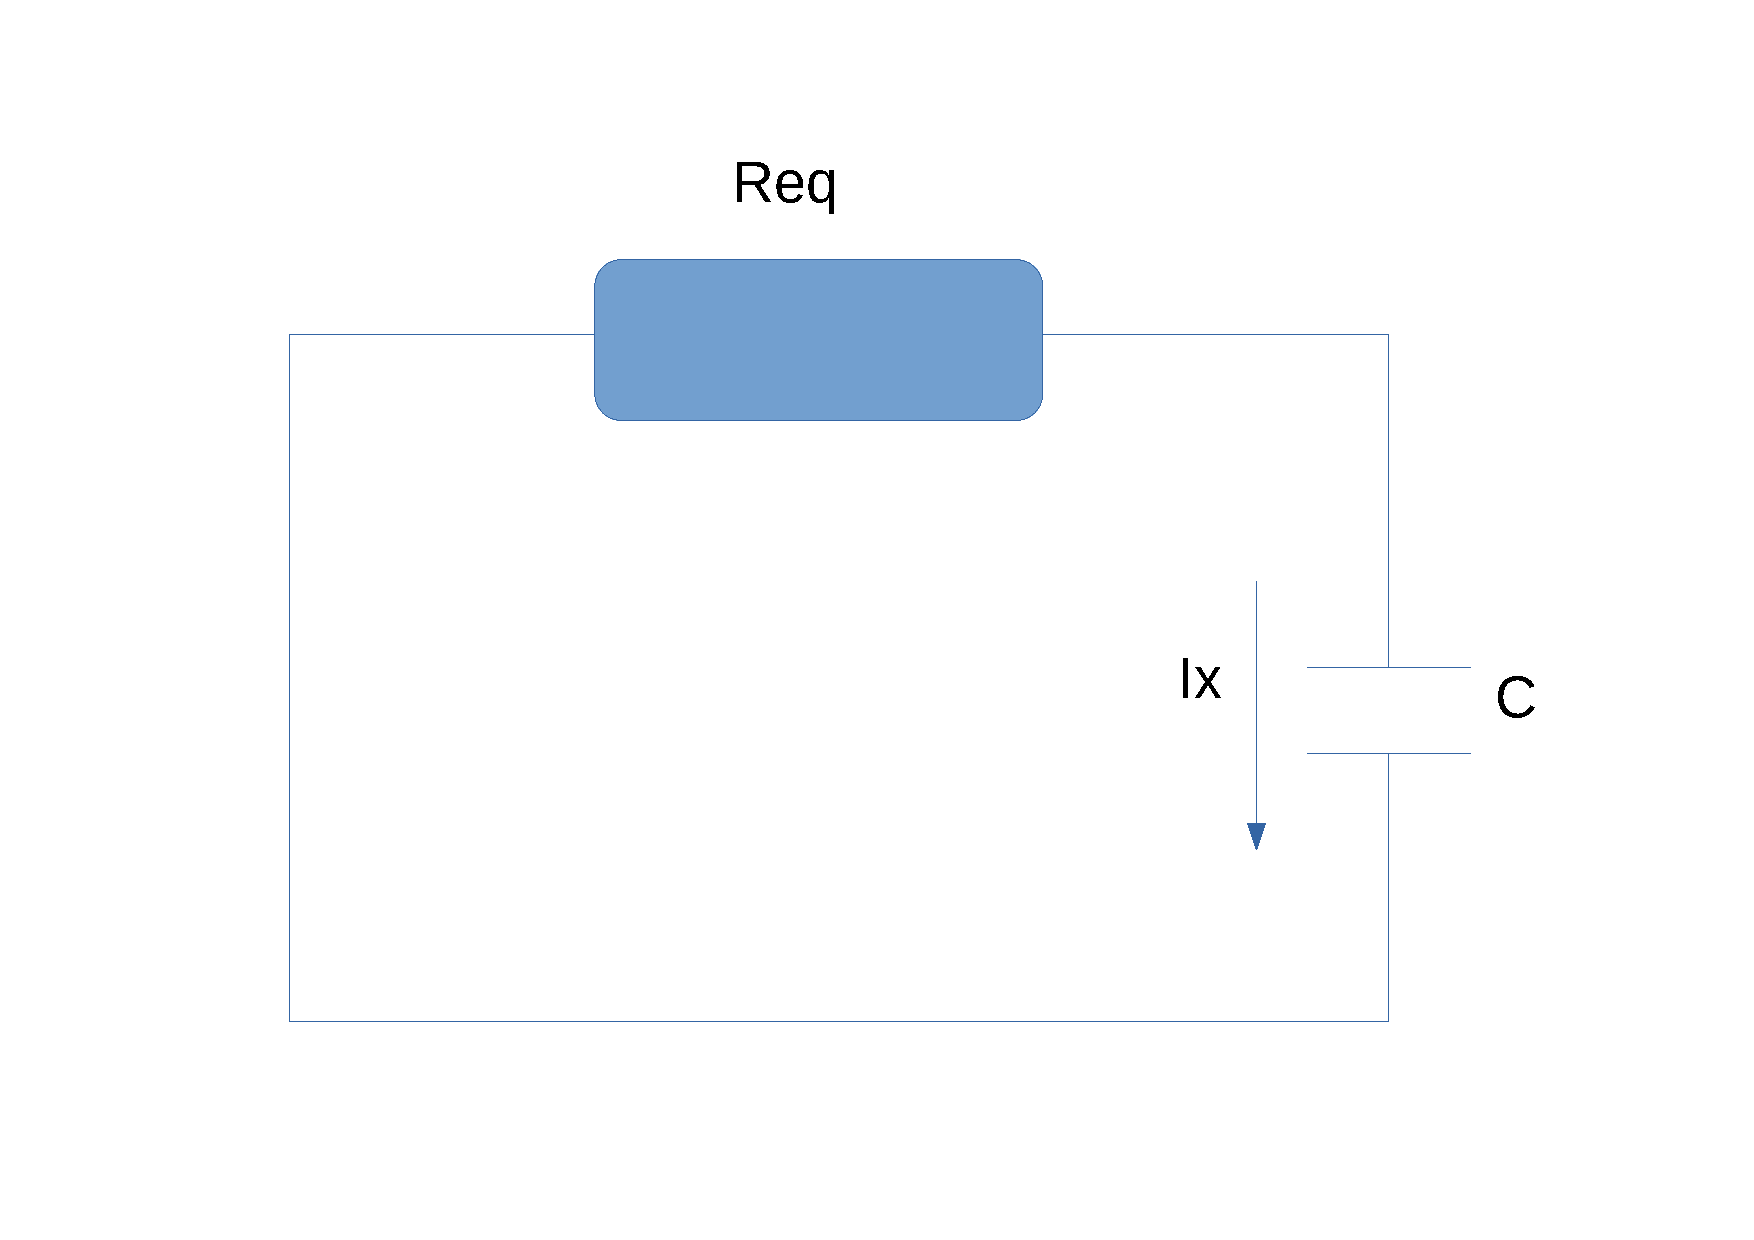
\includegraphics[width=0.5\linewidth]{Circuito3.pdf}
\caption{Third Circuit}
\label{fig:snat}
\end{figure}

\begin{figure}[!h] \centering
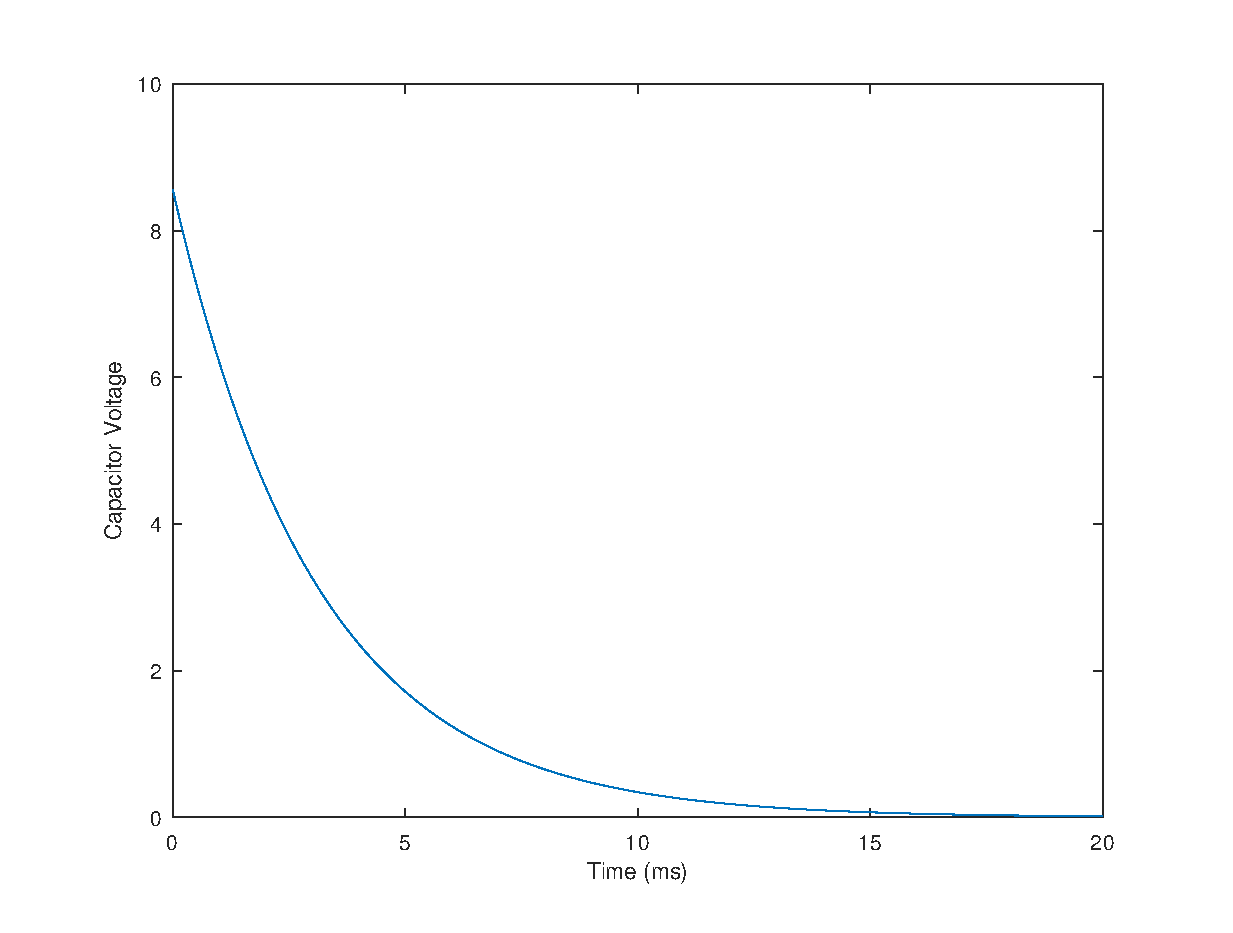
\includegraphics[width=0.7\linewidth]{naturalsolution.eps}
\caption{Natural Solution $v_{6n}(t)$, $t\in[0,20]$ ms}
\label{fig:snat}
\end{figure}


\newpage
\subsection{Forced Solution $V_{6f}$(t), in the interval [0,20]ms}

\par In a forced circuit the voltages in the nodes will have the same frequency as the source. Consequently, the voltage in the node will be something like $V_{node} = V_{node_{max}}*cos(wt + \phi_{node})$. In order to determine the voltages in the nodes, we have to determine their amplitudes and phases. In other words, we have to calculate their complex amplitude. In complex terms, the voltage in the nodes will be in the form $V_{node} =
V_{node_{max}}*e^{wt}*e^{\phi_{node}})$.

\par To obtained this solutions, we rearranged the equations in the matrix form below, in order to find the solution using Octave math tools.

\begin{equation}
    w= 2*\pi*f
\end{equation}

\begin{equation}
    V_C = \frac{1}{j*w*C}
\end{equation}

$\begin{bmatrix}
1 & 0 & 0 & -1 & 0 & 0 & 0 & 0 \\
G_1 & -G_1-G_2-G_3 & G_2 & 0 & G_3 & 0 & 0 & 0\\
0 & K_b+G_2 & -G_2 & 0 & -K_b & 0 & 0 & 0\\
0 & 0 & 0 & 1 & 0 & 0 & 0 & 0\\
0 & G_3 & 0 & G_4 & -G_3-G_4-G_5 & G_5+1/Z_C & G_7 & -G_7-1/Z_C\\
0 & K_b & 0 & 0 & -K_b-G_5 & G_5+1/Z_C & 0 & -1/Z_C\\
0 & 0 & 0 & -G_6 & 0 & 0 & G_6+G_7 & -G_7\\
0 & 0 & 0 & K_d*G_6 & -1 & 0 & -K_d*G_6 & 1\\
\end{bmatrix}$
$\begin{bmatrix}
V_1 \\ V_2 \\ V_3 \\ V_4 \\ V_5 \\ V_6 \\ V_7 \\ V_8
\end{bmatrix}$
= 
$\begin{bmatrix}
1 \\ 0 \\ 0 \\ 0 \\ 0 \\ 0 \\ 0 \\ 0
\end{bmatrix}$

\paragraph{}
\par The tables below contain the amplitudes and the phases of the differents nodes,that allows us to compute the complex amplitude of every node voltage. So, $V_{6} = A*cos(wt + \phi)$, and you can see the amplitude and the phase below.

\begin{table}[!h]
\centering
\begin{tabularx}{0.6\textwidth} {
  | >{\raggedright\arraybackslash}X
  | >{\raggedleft\arraybackslash}X | }
 \hline
V1 & 1.000000e+00 V\\ \hline
V2 & 9.529674e-01 V\\ \hline
V3 & 8.565095e-01 V\\ \hline
V4 & 0.000000e+00 V\\ \hline
V5 & 9.593618e-01 V\\ \hline
V6 & 5.727806e-01 V\\ \hline
V7 & 3.784988e-01 V\\ \hline
V8 & 5.707419e-01 V\\ \hline

\end{tabularx}
\caption{Amplitudes of nodal voltages in V}
\end{table}

\begin{table}[!h]
\centering
\begin{tabularx}{0.6\textwidth} {
  | >{\raggedright\arraybackslash}X
  | >{\raggedleft\arraybackslash}X | }
 \hline
Phase 1 & 0.000000e+00 Radians\\ \hline
Phase 2 & 5.945769e-16 Radians\\ \hline
Phase 3 & 1.711774e-15 Radians\\ \hline
Phase 4 & 0.000000e+00 Radians\\ \hline
Phase 5 & 5.280845e-16 Radians\\ \hline
Phase 6 & -2.991803e+00 Radians\\ \hline
Phase 7 & -3.141593e+00 Radians\\ \hline
Phase 8 & -3.141593e+00 Radians\\ \hline

\end{tabularx}
\caption{Phases of nodal voltages in Rad}
\end{table}

\newpage

\subsection{Final Solution $V_{6}$(t), in the interval [0,20]ms}


\par The total response of a circuit can be seen as the sum of the natural and forced response, using the principle of superposition. These two solution were calculated in the section 2.3 and 2.4.

The final solution for $V_6$(t) is: 

\begin{equation}
    V_{6f} = \begin{cases} V_6, \quad t<0 \\ V_{c}*e^{-\frac{t}{C*R_{eq}}} + A*cos(wt + \phi), \quad t \geq 0  \end{cases}
\end{equation}


The final solution for $V_s$(t) is:

\begin{equation}
    V_{sf} = \begin{cases} V_s, \quad t<0 \\ sin(2 \pi ft), \quad t \geq 0 \end{cases}
\end{equation}

In the following plot you can see this evolutions:

\begin{figure}[!h]\centering
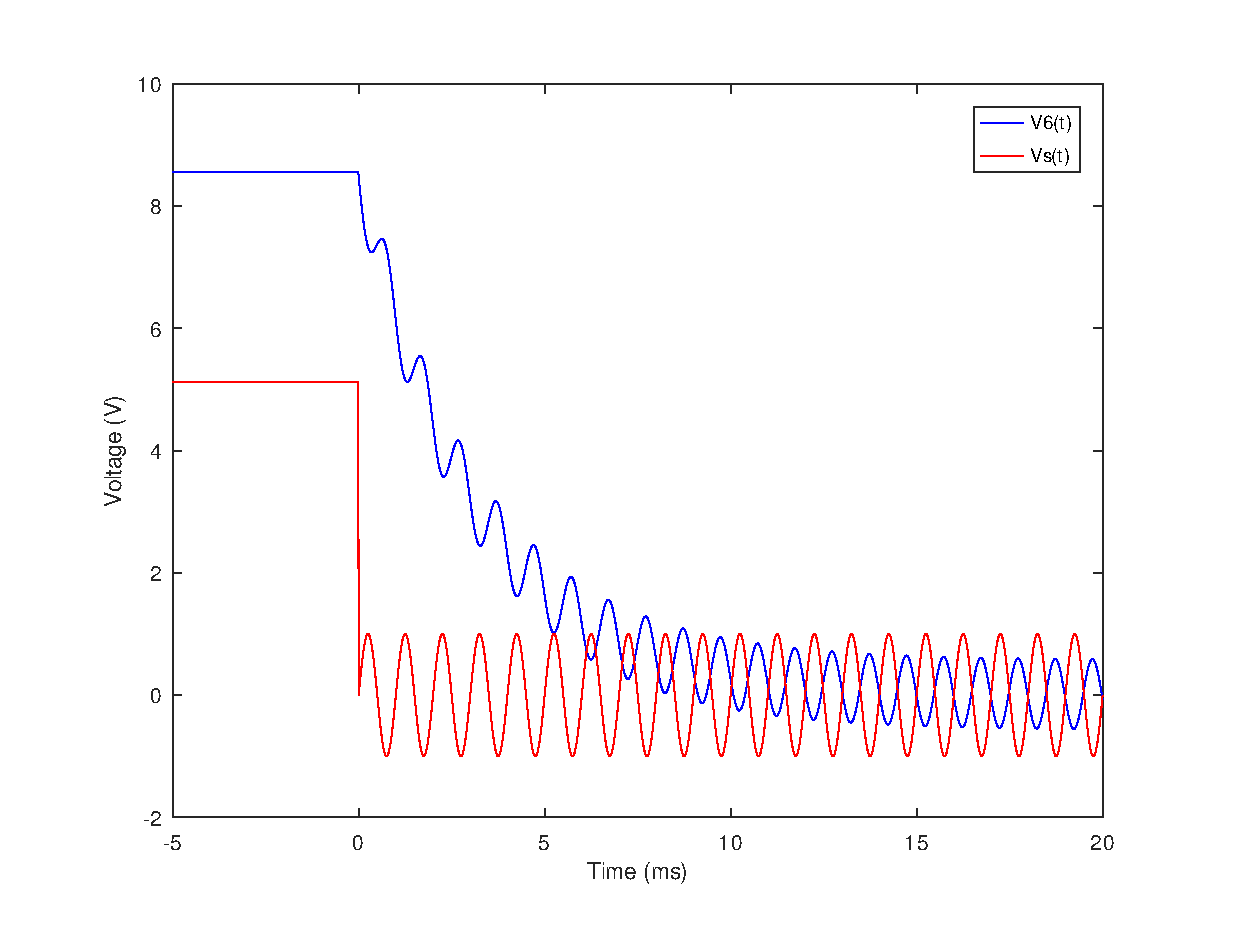
\includegraphics[width=0.7\linewidth]{forced_and_natural_solution.eps}
\caption{Final Solution}
\label{fig:snat}
\end{figure}

\subsection{Frequency response for $V_c$(f), $V_6$(f) and $V_s$(f)}

In this section we determine the frequency responses $V_c(f) = V_6(f) - V_8(f)$ and $V_{6}$(f), for frequency range 0.1Hz to 10MHz. To the magnitude response we use a logscale in order to provide a much better plot fit and a better great visualization for users. The unit of the magnitude is the decibel, which is common used for sound waves. To solve this problem we use the equations rearranged in the matrix in 2.4, in a cycle.


\subsubsection{Magnitude}
The magnitude is in dB, the absolute values were converted ($X_dB=20log10(X)$). The frequencies were put in a logarithmic scale.
The magnitude of $V_s$ is constant despite the variation of the frequency of the signal. Since its amplitude is 1, as one can observe in the graphics shown at the end of the section, the plot shows a constant
horizontal line, with the value zero (0=log10(1)).
On the other hand, as the frequency is increasing, the magnitudes of $V_6$ and $V_c$ decrease. As it is expected in a  RC circuit, due to the capacitor's impedance $(Z_C = 1/j*w*C)$, the value of $V_c$ changes.

\begin{figure}[!h]\centering
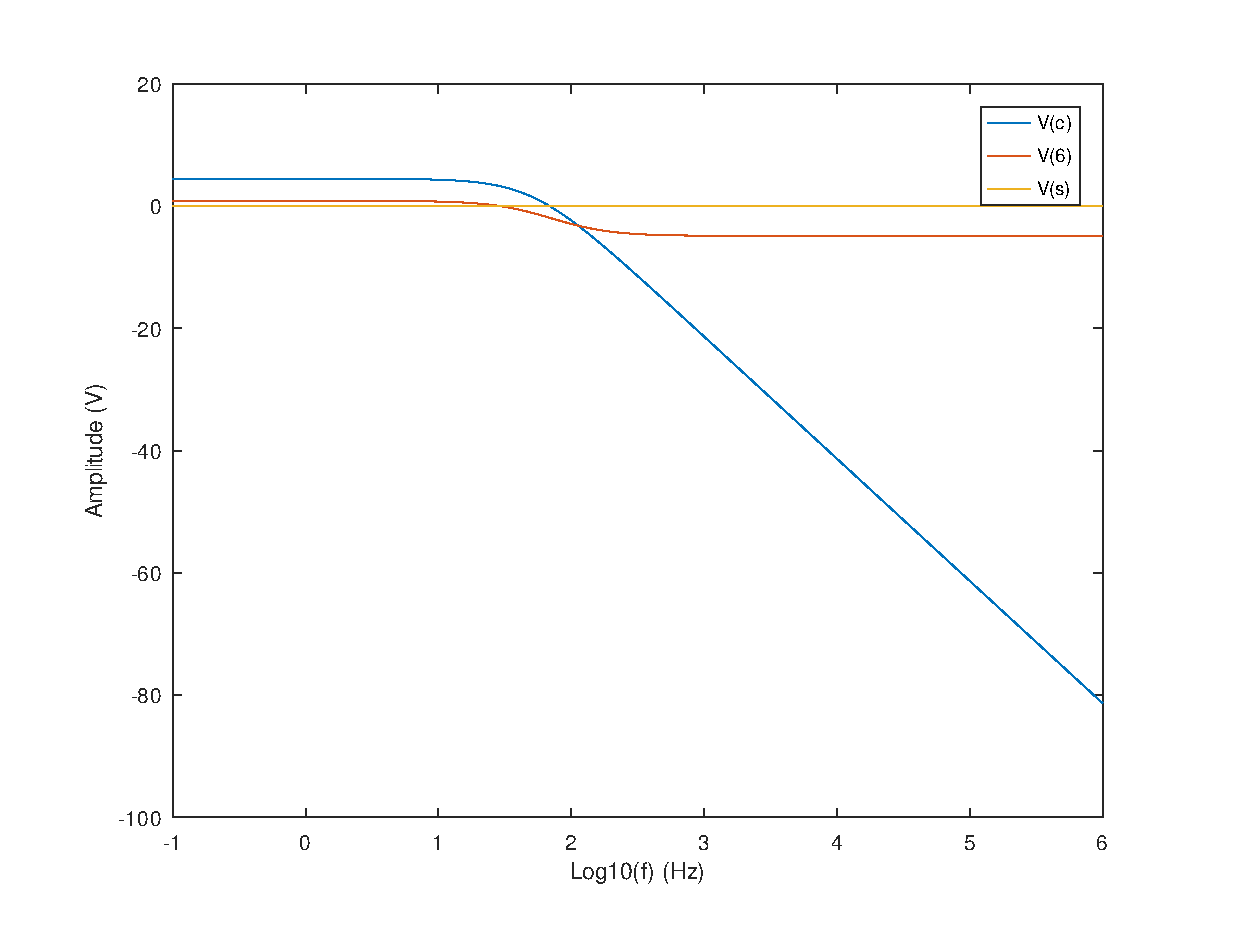
\includegraphics[width=0.5\linewidth]{amplitude.eps}
\caption{Amplitude}
\label{fig:snat}
\end{figure}

\subsubsection{Phase}

The angles are in degrees. As we expected the phase of $V_{s}$ is 0, and the phase of $V_{c}$ tends to -90° and $V_{6}$ to -180°, as the frequency is increasing. In the plot below we can see the evolution.

\begin{figure}[!h]\centering
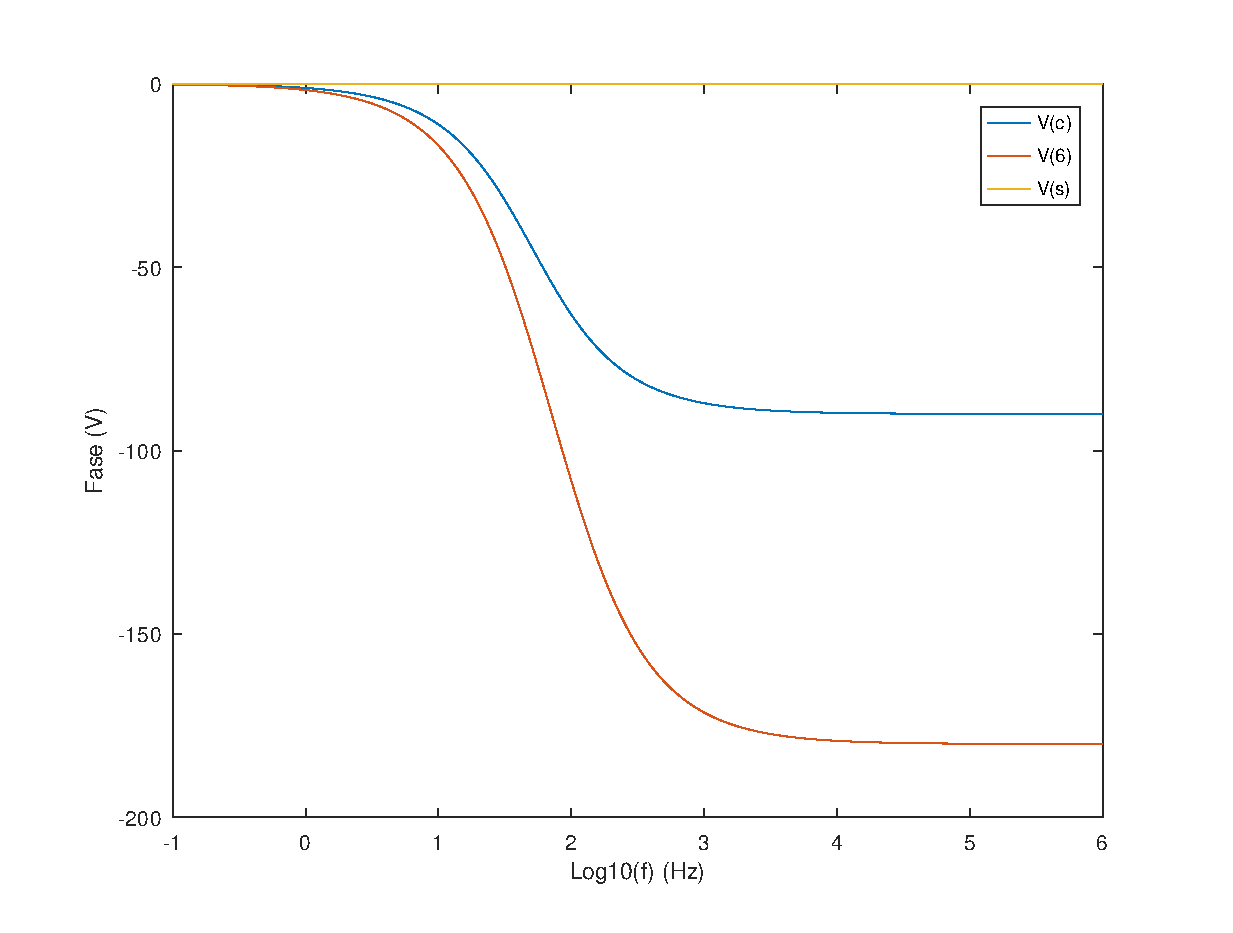
\includegraphics[width=0.5\linewidth]{phase.eps}
\caption{Phase}
\label{fig:snat}
\end{figure}
